\section{Experiment}
\label{sec:experiment}
This section presents citation patterns in representative and widely used GESs within the political domains of Japan and the United States using the methodology proposed in Section~\ref{sec:methodology}.
The purpose of this experiment is twofold: (1) to reveal the potential attack surface of GESs from the perspective of PoisonedRAG attacks in representative and widely used GESs within the political domain, which is critical because these GESs can significantly influence citizens' decision-making in elections, and (2) to accelerate research addressing these risks by sharing the publisher attribute perspective with the research community.
% Accordingly, this study focuses on representative and major closed models, examining questions in the political domain as an exemplar of an urgent and consequential issue through detailed analysis.
Our experimental goal is not to demonstrate effectiveness across exhaustive domains, but rather to illustrate the attack surface and threats that exist in the GESs from the perspective of publisher attributes.

\begin{figure*}[htbp]
\begin{subfigure}[b]{0.32\textwidth}
    \centering
    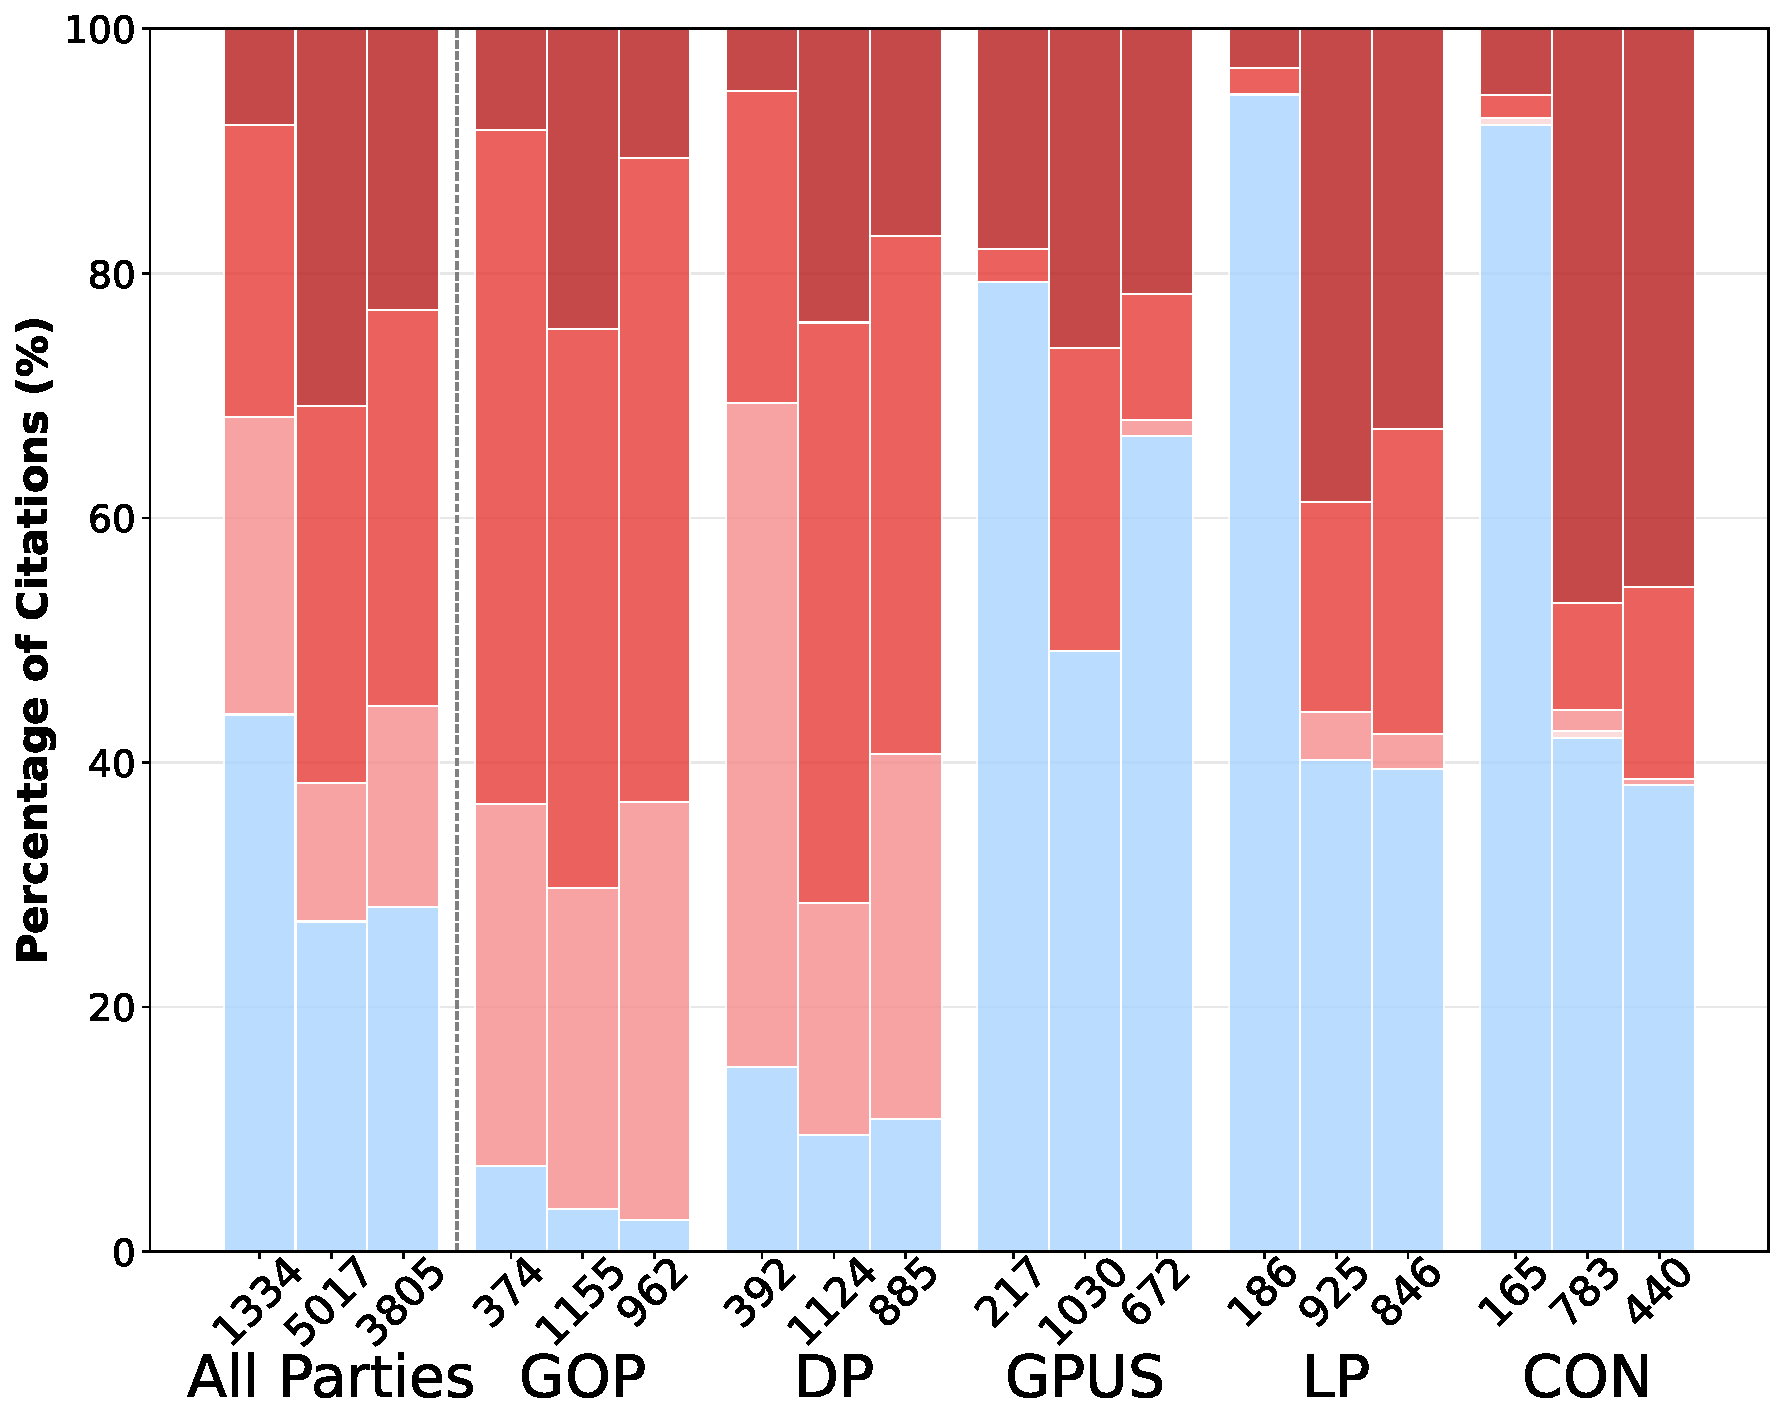
\includegraphics[width=\textwidth]{figs/US/all_parties_models_integrated_en_politics_prompts_red-blue.pdf}
    \caption{Citation Distributions (U.S.)}
    \label{fig:all_en}  
\end{subfigure}
\begin{subfigure}[b]{0.64\textwidth}
    \centering
    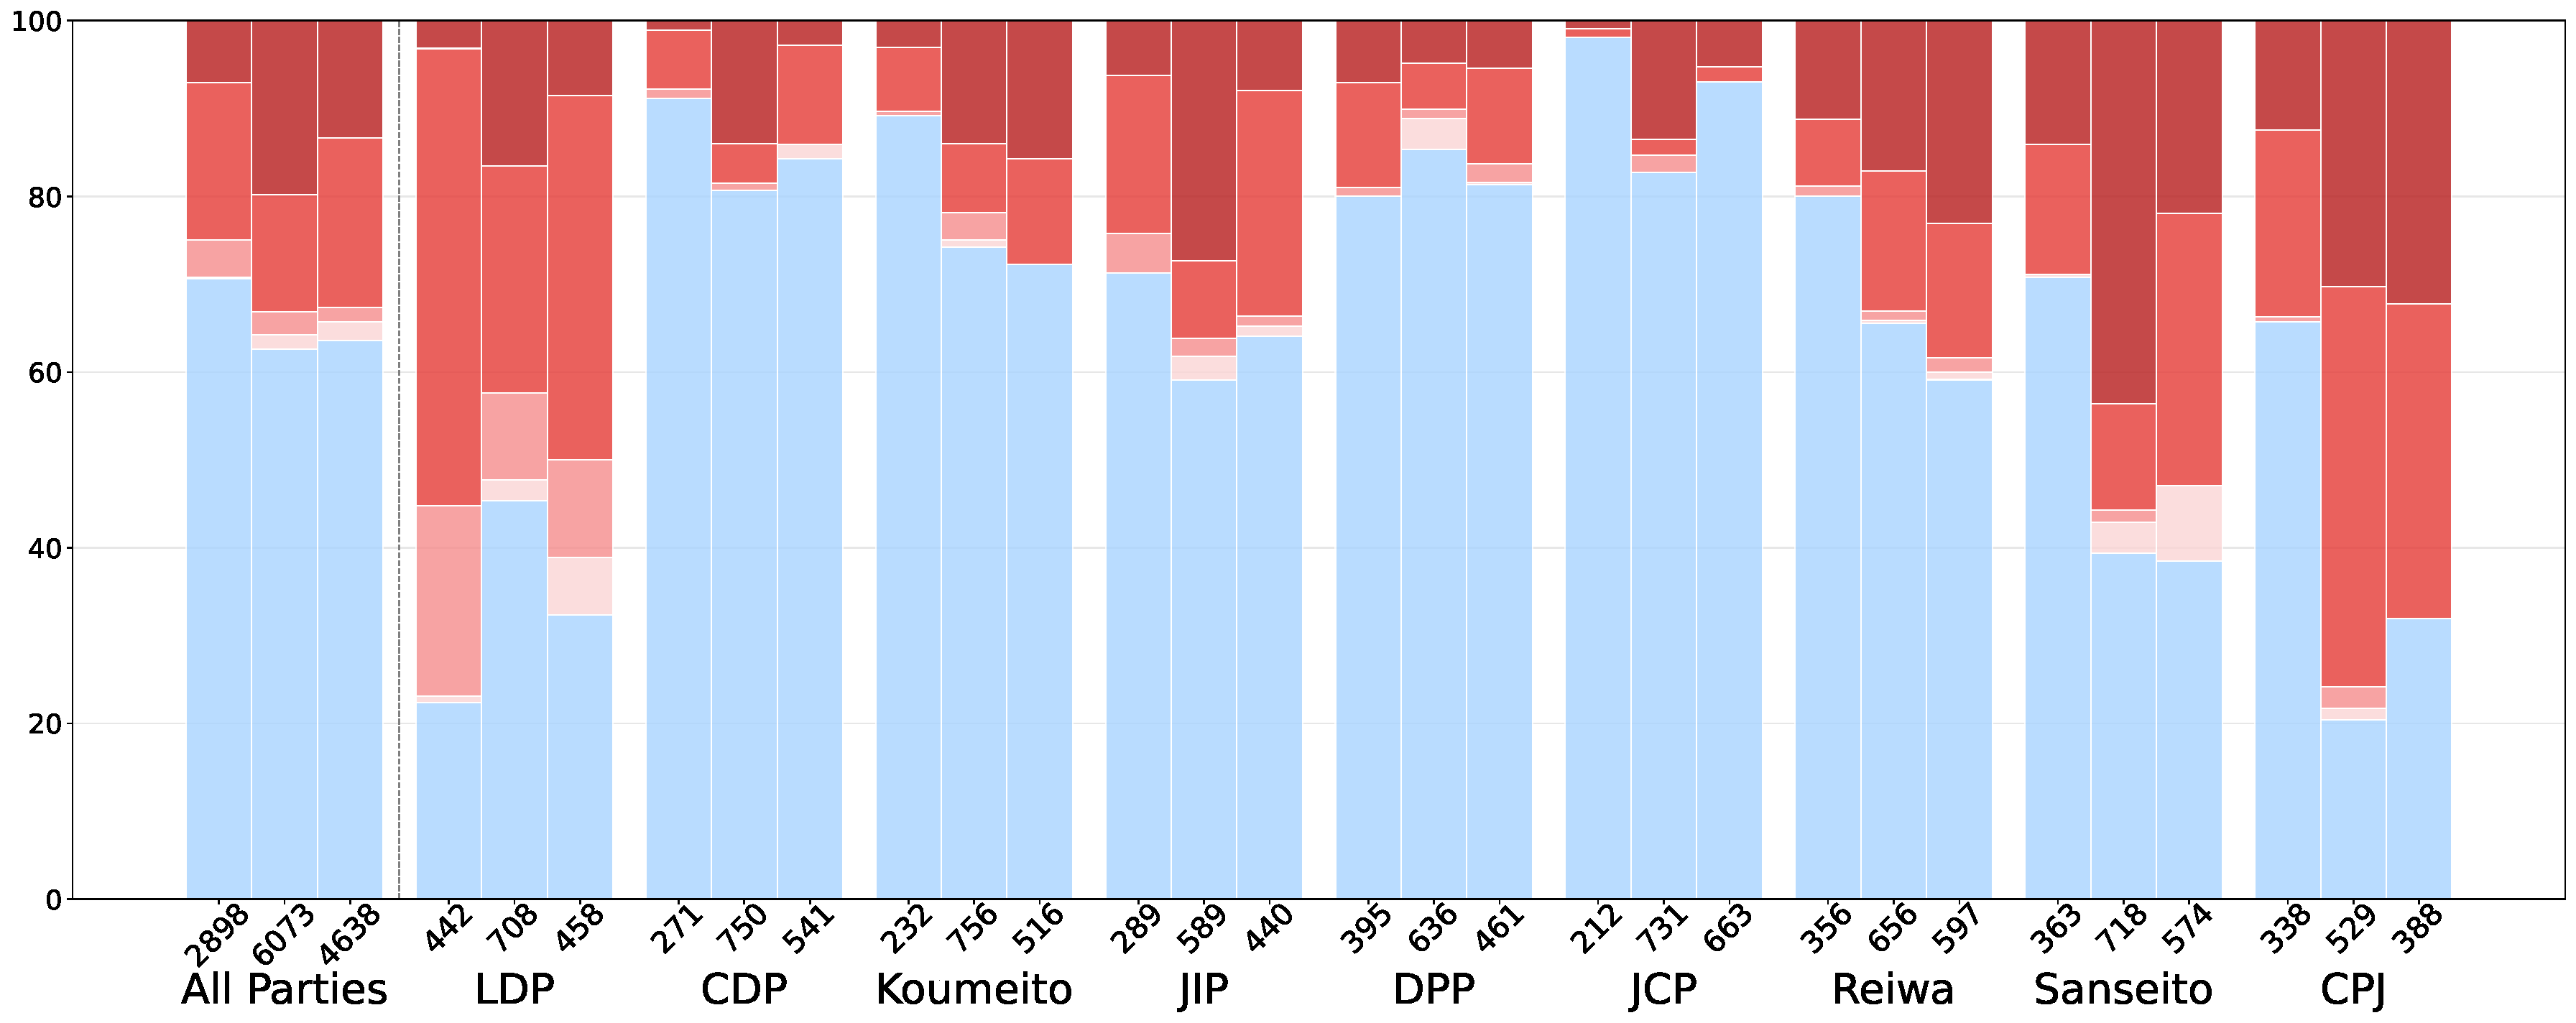
\includegraphics[width=\textwidth]{figs/JA/all_parties_models_integrated_ja_politics_prompts_red-blue.pdf}
    \caption{Citation Distributions (Japan)}
    \label{fig:all_ja}
\end{subfigure}
\begin{subfigure}[b]{0.99\textwidth}
    \centering
    
\includegraphics[width=\textwidth]{figs/full_legend.pdf}
\end{subfigure}
\caption{Distribution of citation sources by party in the US (a) and Japan (b): Each stacked bar shows the proportion of cited sources (primary, opponent, and secondary information sources categorized by attack cost) for responses generated by different APIs.
For each party, the three adjacent bars correspond to results from OpenAI (left), Gemini (middle), and Claude (right).
The three bars on the far right of each panel show aggregated results across all parties. The ``opponent source'' in All Parties chart reffers to the citation sources from parties that are not the target party for each question. The numbers under each chart shows the amout of total citation constructing it.}
\label{fig:party_wise}
\end{figure*}

\subsection{Experimental Setup}
We focus on the political domain because the flow of information from political parties to citizens constitutes a cornerstone of democratic electoral processes~\cite{the-trust-gap-young-peoples-tactics-for-assessing-the-reliability-of-political-news-ijpp22, kovach2007elements}.
Contemporary elections depend critically on digital information dissemination, and citizens increasingly rely on GESs to gather information that shapes their voting decisions.
GESs can significantly influence citizens' decision-making, rendering the threat of PoisonedRAG attacks particularly severe in this domain.
We emphasize that our experiment aims to measure actual citation patterns in the political domain rather than prescribe ideal proportions; we defer discussion of desirable citation balance for GESs to Section~\ref{sec:discussion}.

We design political questions about topics common to both countries and generate answers to those questions.
We prepare ten policy questions and ten ideology questions, totaling twenty questions.
All questions are closed-ended and include a party name according to PoisonedRAGs study (e.g, ``Regarding government debt, does {PARTY} currently prioritize debt restraint or growth-oriented investment?'').
We show all questions in our repository~\cite{QL_CIKM_RERO}.
The scale of our question set is comparable to seminal evaluation studies, which typically use \(50\)--\(100\) questions (e.g., Guan et al.~\cite{guan2024language}; Wang et al.~\cite{wang2024factcheck}).

We clarify that our questions are designed to elicit policy positions without bias toward specific parties.
Our questions are designed to be politically neutral, focusing on whether GESs cite contents that articulate positions on the target topics rather than favoring any particular party; consequently, our findings reflect citation patterns rather than biases introduced by question design.
The questions are prepared in two languages: Japanese for Japanese politics and English for U.S. politics.
Answers to Japanese questions are generated in Japanese, and answers to U.S. questions are generated in English.

We target political parties that satisfy each country's requirements for national political parties as primary information sources.
Specifically, in Japan we target nine parties: ``Liberal Democratic Party (LDP)'', ``Constitutional Democratic Party of Japan (CDP)'', ``Komeito'', ``Japan Innovation Party (JIP)'', ``Democratic Party for the People (DPP)'', ``Japanese Communist Party (JCP)'', ``Reiwa Shinsengumi (Reiwa)'', ``Sanseito'', and ``Conservative Party of Japan (CPJ)''; in the U.S. we target five parties: ``Republican Party (GOP)'', ``Democratic Party (DP)'', ``Green Party (GPUS)'', ``Libertarian Party (LP)'', and ``Constitution Party (COP)''.
We prepare twenty questions for each party, resulting in \(180\) questions for Japan and \(100\) questions for the U.S. respectively.

We employ three GES models for answer generation: OpenAI GPT-5~\cite{chatgpt}, Claude Sonnet \(4\) (claude-4-sonnet-20250514)~\cite{claude}, and Gemini Flash \(2.0\) (gemini-2.0-flash)~\cite{gemini}, the most advanced publicly available models with web search mode enabled.
We clarify why we focus on closed GES models in this study.
According to surveys~\cite{menlo-ventures2025stategenaienterprise, a16z2025stateconsumerai}, closed models dominate the LLM market in both enterprise and consumer segments, with Claude, OpenAI, and Gemini together accounting for 88\% of spending share, while open-source models account for only 11\%.
These models are developed in the U.S., but they dominate usage in Japan as well.
According to GMO Research \& AI~\cite{gmo-research2025japanai}, Japanese users predominantly rely on closed models such as GPT, Gemini, and Copilot, all of which are U.S.-developed products.
While Japan has developed numerous LLM models, to our knowledge, no Japanese GES models are publicly available.
Furthermore, widely deployed GESs such as Google AI Overview, which integrates Google Search by default, rely on the closed model Gemini~\cite{stein2025expandingaioverviewsaimode, reid2025aisearchbeyondinformation}; consequently, users routinely encounter generated answers from closed GES models when conducting web searches, underscoring the central role these models play in contemporary information retrieval.
Note that we do not limit our evaluation criteria to closed models because our evaluation criteria do not use the internal reasoning states of GESs but only use input and output of GESs (question and answer).
To provide reproducibility, the question-answer datasets are available in our repository~\cite{QL_CIKM_RERO}.

In our experiments, the temperature of each GES model cannot be set because APIs do not allow setting temperature for LLMs with search mode enabled; thus, the cited web sources and textual content of answers vary across generations.
To capture answer variation, we ask each question five times to suppress bias from a single answer.
The answers are obtained on September \(4\), \(2025\).


\subsection{Distribution of Content-injection Barriers in Answers}
\label{sec:api_response}
This sub-experiment answers which publisher attributes from the perspective of content-injection barriers GESs preferentially cite (\emph{R-1}).
% To do this, we use citation classification and distribution of content-injection barriers method in Section~\ref{subsec:citation_classification}.
We calculate the proportion of each content-injection barrier using the citation classification method in Section~\ref{subsec:citation_classification} as \( P_{\lambda_i} = |C^{\lambda_i}|/|C| \), where \( |C^{\lambda_i}| \) is the number of citations in content-injection barrier \( \lambda_i \) and \( |C| \) is the total number of citations.

We show the aggregated results in Figures~\ref{fig:all_en}--\ref{fig:all_ja}.
These figures present stacked proportions by party and model.
Each group of three stacked bar graphs shows the proportions of publisher attribute categories of citation web sources in the answer on the horizontal axis.
For each party, the stacks are ordered left to right as OpenAI, Gemini, and Claude, respectively.
The three graphs at the left edge of each figure show the combined results of all citations across parties as a baseline for each model.

We first analyze the overall trends in citation patterns.
Overall, for Japanese questions (Japanese parties), all three models show a high proportion of target-party primary information sources, accounting for about \(60\%\): OpenAI \(63.0\%\), Gemini \(60.9\%\), and Claude \(60.9\%\).
In contrast, for U.S. questions (U.S. parties), the proportion of primary information sources decreases (OpenAI \(43.9\%\), Gemini \(27.0\%\), Claude \(28.1\%\)), and the proportion of secondary information sources increases.
We observe a large structural difference: primary source dependence in the Japanese setting and external source dependence in the U.S. setting.

We observe distinct differences in citation patterns across the three models.
Gemini consistently exhibits strong platform dependence: low-barrier sources contribute \(19.9\%\) in Japanese questions and \(30.9\%\) in U.S. questions.
Claude tends to use media-related sources the most: medium-barrier sources contribute \(19.3\%\) in Japanese questions and \(32.3\%\) in U.S. questions.
OpenAI cites categories in a more balanced manner: medium-barrier sources \(17.7\%\) and low-barrier sources \(7.2\%\) in Japanese questions, whereas high-barrier sources \(24.3\%\) and medium-barrier sources \(23.9\%\) in U.S. prompts.
Gemini is platform-leaning, Claude is media-leaning, and OpenAI is distributed.

We identify significant differences in citation patterns between Japanese and U.S. contexts.
With Japanese questions, all three models converge to around a \(60\%\) share for primary information sources, and opponents and secondary information sources are used in a supplementary role.
With U.S. questions, the share of primary information sources falls to the \(20\%\)--\(40\%\) range, and the shortfall is supplemented by different opponent and secondary information sources depending on the model.
Concretely, in the U.S., Gemini emphasizes platform sources (\(30.9\%\)), Claude emphasizes media sources (\(32.3\%\)), and OpenAI emphasizes high-barrier sources (\(24.3\%\)), indicating that the direction of external dependence diverges substantially by country and language.

We examine citation patterns for individual U.S. political parties.
For both the Republican and Democratic Parties, the two major parties in the U.S., the proportion of opponents and secondary information sources is high across models, with medium- and high-barrier sources as the main components.
Except for questions about the Democratic Party with OpenAI, the two parties often cite low- and medium-barrier sources.
In contrast, the Green Party frequently cites low-barrier sources.
Other parties tend to cite official party sources more, though the volume varies across models and parties.
For the Green Party, OpenAI and Claude have high shares of primary information sources (\(80\%\) and \(70\%\), respectively), whereas for Gemini roughly \(10\%\) of that share is replaced by medium-barrier sources.
For the Libertarian Party and the Constitution Party, similar tendencies are observed: only OpenAI shows a remarkably high share (greater than \(90\%\)) from primary information sources, whereas other models increase dependence on low-barrier sources to around \(40\%\).

We analyze citation patterns for individual Japanese political parties.
The current ruling party, the Liberal Democratic Party, shows a mitigated concentration on primary information sources compared with other parties.
Meanwhile, citations from high-barrier sources, which are opponents and secondary information sources with high barriers, increase; nevertheless, compared with questions about other parties, citations from high-barrier opponents and secondary information sources remain relatively high.
For the Constitutional Democratic Party of Japan, Komeito, and the Japan Innovation Party, primary information sources generally account for \(70\%\)--\(90\%\), and secondary information sources remain supplementary.
The Japanese Communist Party exhibits particularly high dependence on the party's official domain, with answer justifications concentrating in intra-party information.
For Sanseito and the Conservative Party of Japan, the shares from platforms and media increase relatively in Gemini and Claude, indicating a structure in which the shortage of party primary information sources is supplemented by opponents and secondary information sources.
Looking at the results for the Liberal Democratic Party in Japan and the Republican Party and Democratic Party in the U.S., questions about the major parties in their countries tend to have low citations from primary information sources.
This could be because those parties are major parties in their countries, and there may be influence from the vast number of secondary information sources, especially in government and media domains.

\begin{figure*}[htbp]
    \centering
    \vspace{1em}
    \begin{subfigure}[t]{0.32\textwidth}
        \centering
        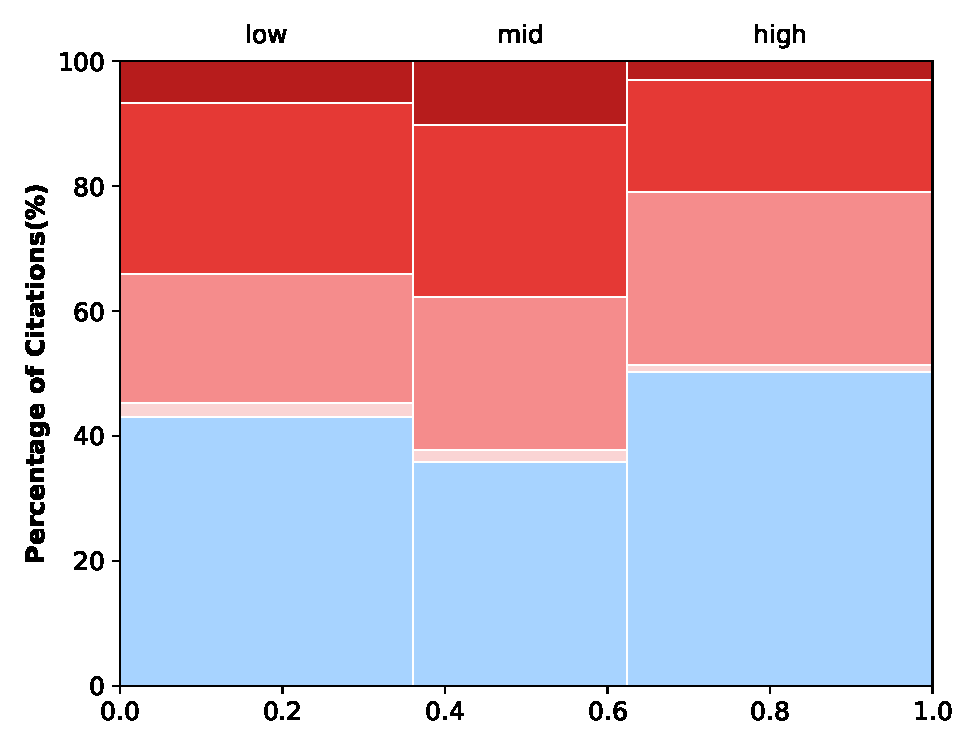
\includegraphics[width=\textwidth]{figs/coverage/citation_ratio_mekko_session-en_politics_prompts_model-openai_target-all_category-all_red_blue.pdf}
        \caption{Distributions in OpenAI (U.S.)}
        \label{fig:citation_coverage_en_openai}
    \end{subfigure}
    \begin{subfigure}[t]{0.32\textwidth}
        \centering
        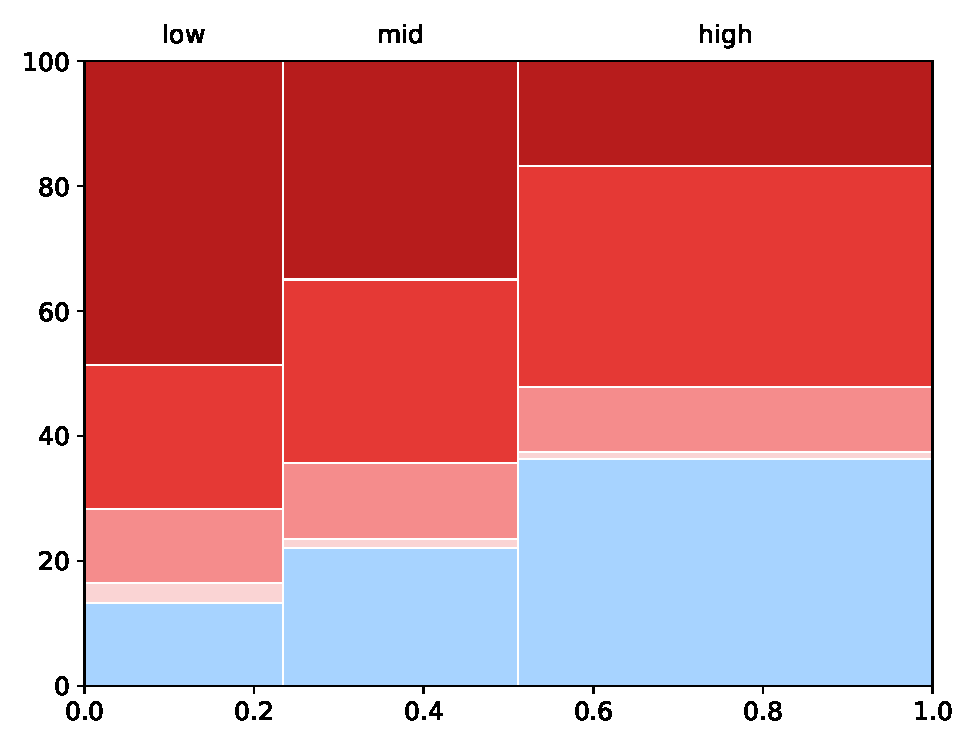
\includegraphics[width=\textwidth]{figs/coverage/citation_ratio_mekko_session-en_politics_prompts_model-gemini_target-all_category-all_red_blue.pdf}
        \caption{Distributions in Gemini (U.S.)}
        \label{fig:citation_coverage_en_gemini}
    \end{subfigure}
    \begin{subfigure}[t]{0.32\textwidth}
        \centering
        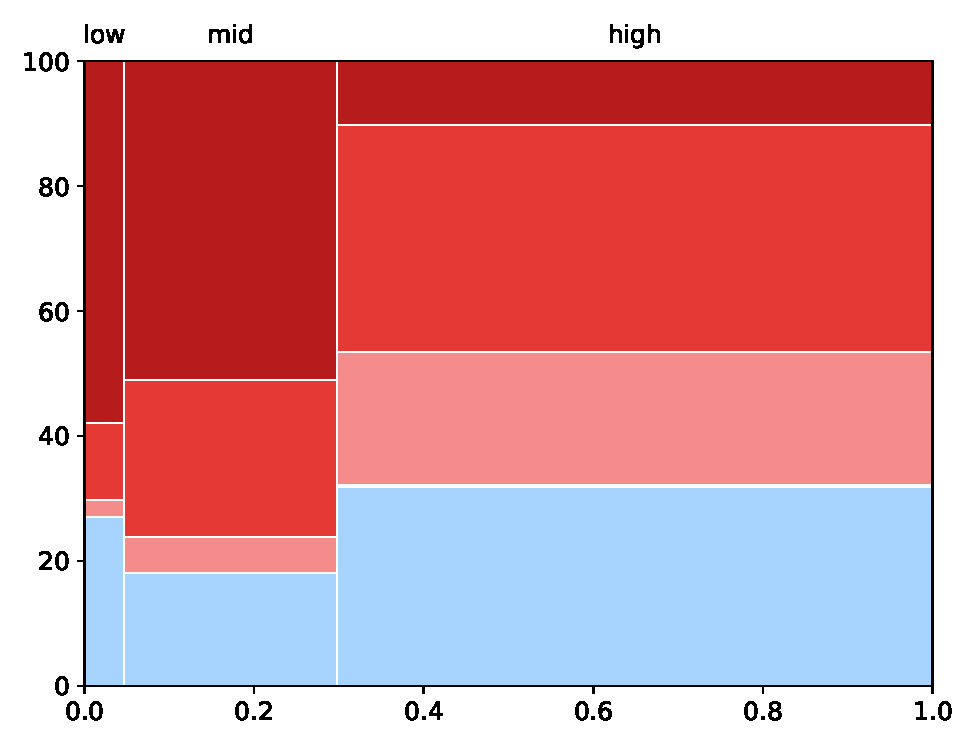
\includegraphics[width=\textwidth]{figs/coverage/citation_ratio_mekko_session-en_politics_prompts_model-claude_target-all_category-all_red_blue.pdf}
        \caption{Distributions in Claude (U.S.)}
        \label{fig:citation_coverage_en_claude}
    \end{subfigure}
    \begin{subfigure}[t]{0.32\textwidth}
        \centering
        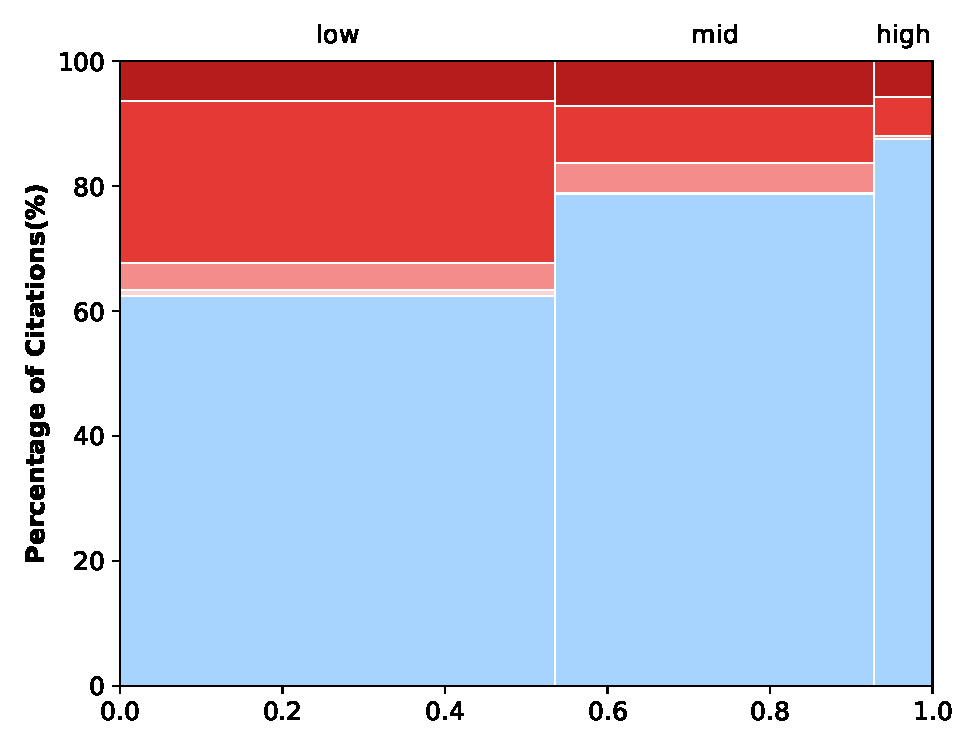
\includegraphics[width=\textwidth]{figs/coverage/citation_ratio_mekko_session-ja_politics_prompts_model-openai_target-all_category-all_red_blue.pdf}
        \caption{Distributions in OpenAI (Japan)}
        \label{fig:citation_coverage_ja_openai}
    \end{subfigure}
    \begin{subfigure}[t]{0.32\textwidth}
        \centering
        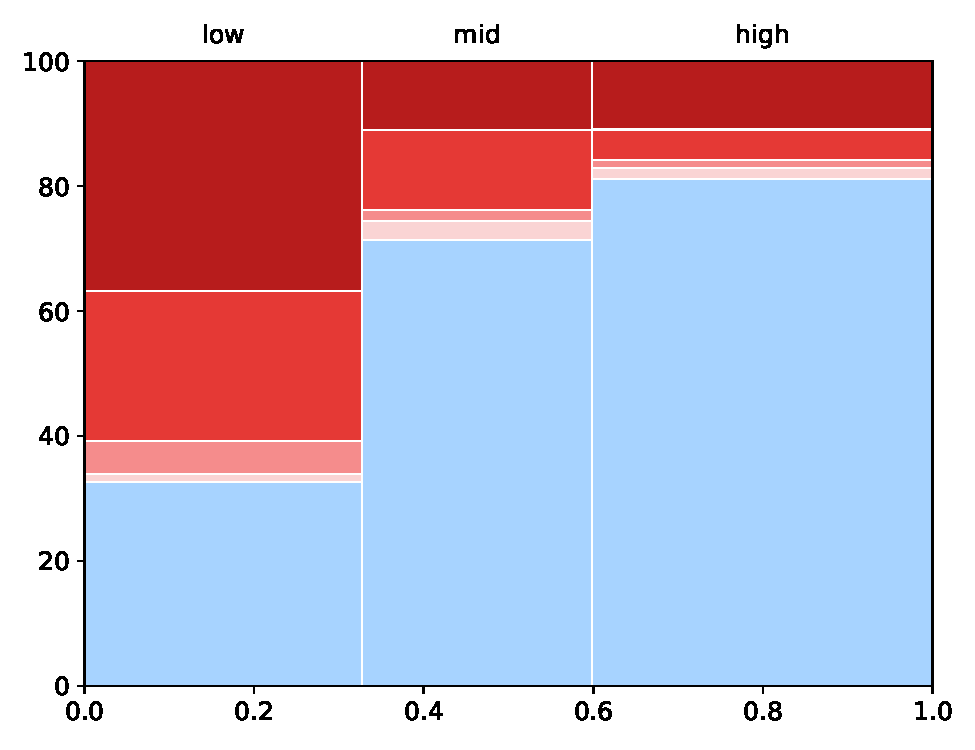
\includegraphics[width=\textwidth]{figs/coverage/citation_ratio_mekko_session-ja_politics_prompts_model-gemini_target-all_category-all_red_blue.pdf}
        \caption{Distributions in Gemini (Japan)}
        \label{fig:citation_coverage_ja_gemini}
    \end{subfigure}
    \begin{subfigure}[t]{0.32\textwidth}
        \centering
        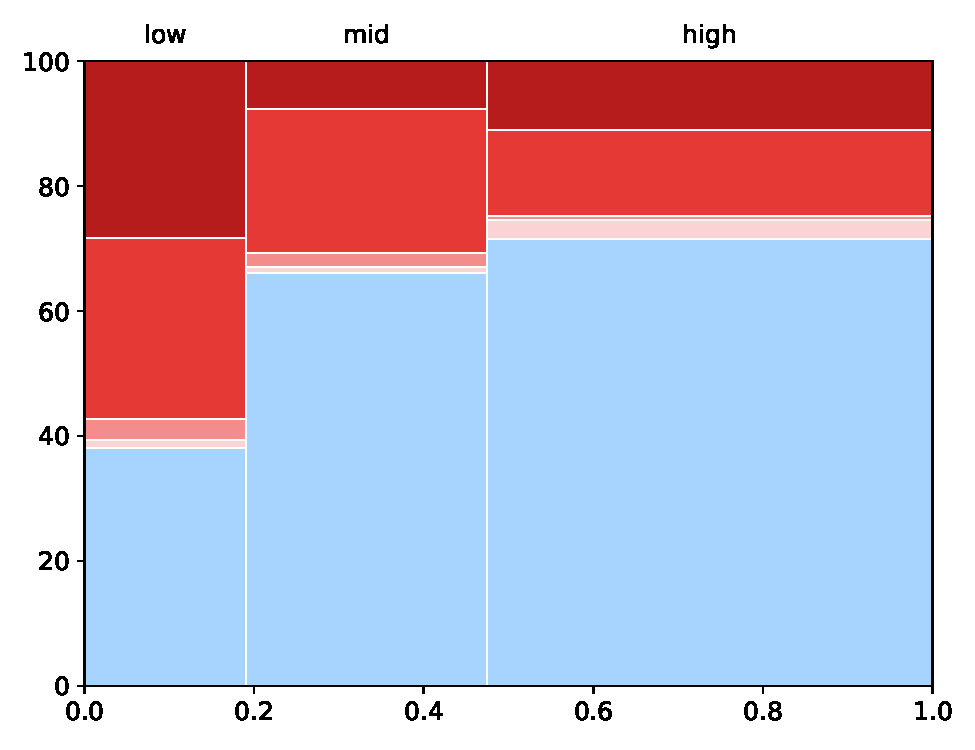
\includegraphics[width=\textwidth]{figs/coverage/citation_ratio_mekko_session-ja_politics_prompts_model-claude_target-all_category-all_red_blue.pdf}
        \caption{Distributions in Claude (Japan)}
        \label{fig:citation_coverage_ja_claude}
    \end{subfigure}
    \begin{subfigure}[t]{0.99\textwidth}
        \centering
        
\includegraphics[width=\textwidth]{figs/full_legend.pdf}
    \end{subfigure}
    \caption{Citation coverage by similarity level for Japanese and English political prompts across models: Each chart shows the distribution of citation source types (primary, opponent, and secondary information sources categorized by attack cost) across three similarity levels(low = [-1.0, 0.8], mid = (0.8, 0.9], and high = (0.9, 1.0]).}
    \label{fig:citation_coverage}
\end{figure*}

\subsection{Distribution of Citation Reflection Power by Content-injection Barriers}
This sub-experiment answers which publisher attributes from the perspective of content-injection barriers GESs preferentially and faithfully reflect in generated answers (\emph{R-2}).
% To do this, we use the citation reflection method in Section~\ref{subsec:citation_reflection}.
For each answer \( r \) under all similarity bands \( b \) and content-injection barrier \( \lambda_i \), we calculate the total count \( N^{(b)}_{\lambda_i} = |\{c_i \in C \mid \psi_{\mathcal{P}}(c_i) = \lambda_i, \tau(c_i, r) = b\}| \) and proportion \( P^{(b)}_{\lambda_i} = N^{(b)}_{\lambda_i}/\sum_{\lambda} N^{(b)}_{\lambda} \) within each band using the classification method \(\psi_{\mathcal{P}}(c_i)\) in Section~\ref{subsec:citation_classification} and the citation reflection \(\tau(c_i, r)\) in Section~\ref{subsec:citation_reflection}.
% We show the aggregated results in Figures~\ref{fig:citation_coverage_en_openai}--\ref{fig:citation_coverage_ja_claude}.

We show the proportion of content-injection barriers within the similarity bands in Figures~\ref{fig:citation_coverage_en_openai}--\ref{fig:citation_coverage_ja_claude}.
The figure shows how content-injection barriers of citations are distributed across these similarity levels using a Marimekko chart.

We examine overall trends in citation reflection coverage across similarity bands.
Comparing the distribution of the coverage between questions about Japanese and U.S. parties, we find that, in both settings, the proportion of highly reliable sources such as primary information sources and high-barrier sources has the greatest coverage in high-similarity bands, whereas the share of opponent and secondary information with medium to low barriers shrinks.
This tendency is common to all models, indicating that high-similarity citations are more strongly supported by primary or high-barrier information.
In contrast, in the low-similarity bands, references originating from opponent and secondary information sources with medium to low barriers are prominent, forming a citation structure where the link between answer sentences and cited sentences is weak.

We analyze model-specific characteristics in citation coverage.
Clear differences exist in the distributions by model.
In the U.S., the \(\geq 0.90\) band expands in all models, securing high similarity not only with primary information sources but also in parallel with opponent sources and high-barrier sources.
In Japan, however, OpenAI has a notably narrow \(\geq 0.90\) band, with most citations concentrated in the low-similarity band (\([-1.0, 0.8]\)).
Gemini shows the clearest tendency to increase the proportion of primary information sources and decrease that of low-barrier sources as the similarity rank increases.
Claude forms high-similarity bands as the main component in both countries; in Japan, primary information sources dominate the high-similarity bands, whereas in the U.S., medium- to high-barrier sources contribute substantially, making co-existence with opponent and secondary information sources conspicuous.

We compare citation coverage patterns between Japan and the U.S.
With questions about Japanese politics, all models show a tendency to increase the proportion of primary information sources and decrease those of low- to medium-barrier sources as the similarity rank increases.
With questions about U.S. politics, by contrast, even in the high-similarity bands the shares of opponent and secondary information sources such as medium- and high-barrier sources are large, and the share of primary information sources is limited.
This difference likely reflects the depth of policy explanations on official party domains and differences in the surrounding external knowledge infrastructure (e.g., government statistics, think tanks, major media, aggregation platforms), as discussed in Section~\ref{sec:api_response}.

These results show that citation coverage serves not merely as a similarity metric but, by indicating which publisher attribute categories have the power to generate the answer, can reveal a model's strategy and the characteristics of the information ecosystem by country.
In Japan, high similarity tends to be supported by dependence on target-party primary information sources, whereas in the U.S., high-barrier opponent and secondary information sources actively contribute to the formation of high similarity.
% Broadly speaking, GESs tend to reflect cited contents more accurately as the reliability of the sources is high.
% This suggests that LLMs take into account the nature of the information originator when deciding the extent to which cited sources are reflected in the answers.
